%%%%%%%%%%%%%%%%%%%%%%%%%%%%%%%%%%%%%%%%%%%%%%%%%%%%%%%%%%%%%
%% APPENDICES
%%%%%%%%%%%%%%%%%%%%%%%%%%%%%%%%%%%%%%%%%%%%%%%%%%%%%%%%%%%%%
\appendix

\chapter{Appendix}
\label{app:acronyms}
%% acronyms
\printindex
\printglossaries

\section{Data sets/Statistical Overview}
\label{app:data_sets}

\begin{comment}
Amount of features before anything was done to the text: 69766 - CountVectorizer(analyzer='word') - \%
Amount of features after adding stop word (English): 69462 - CountVectorizer(analyzer='word', stop\_words="english") - \%
Amount of features after removing code samples, hexadecimals and numeric values: 27624 - \%
Amount of features after setting minimum document frequency: 440 - CountVectorizer(analyzer='word', min\_df=0.01, stop_words='english') - \%


Originally tagged questions as good/bad, but then switched to +/-1 due to considering switching to LibSVM.
\end{comment}

\newpage
\section{MySQL Database}
\label{app:mysql_database}
\begin{figure}[ht]
	\centering
    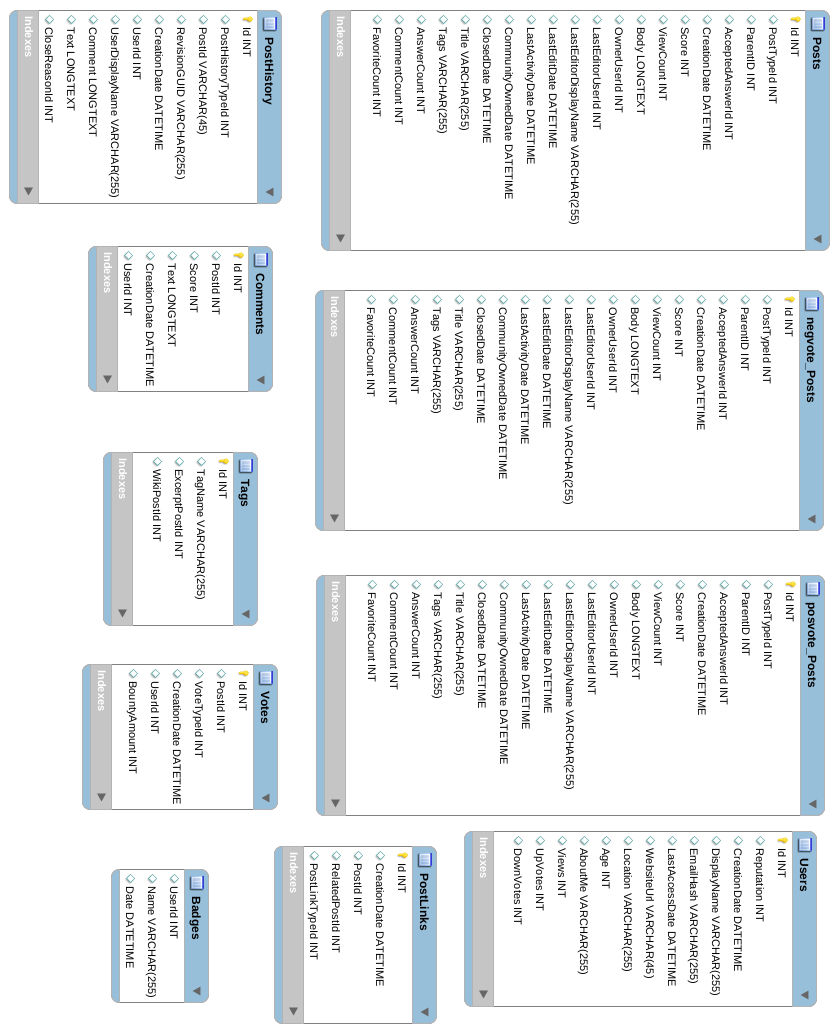
\includegraphics[width=0.8\textwidth]{so_database}
	\caption{MySQL Database used for dataset}
	\label{fig:mysql_database}
\end{figure}